In $h$-multigrid, the different grids have the same polynomial order of finite elements but these elements are amalgamated into increasingly larger elements.
For LFA of $h$-multigrid, we introduce the concept of macro-element bases.
With macro-element bases, the grid transfer operators can be still represented elementwise and can thus be easily represented in the form of Equation \ref{eq:libceed_representation}.

A macro-element basis is formed by amalgamating two or more finite element bases.
Each sub-element has separate quadrature spaces, so the basis functions for each sub-element, are defined as zero on the portions of the domain not included in the given sub-element.
In effect, the basis interpolation and gradient operations for the macro-element provide a sub-element restriction and sub-element basis operation together.

\begin{figure}[!ht]
  \centering
  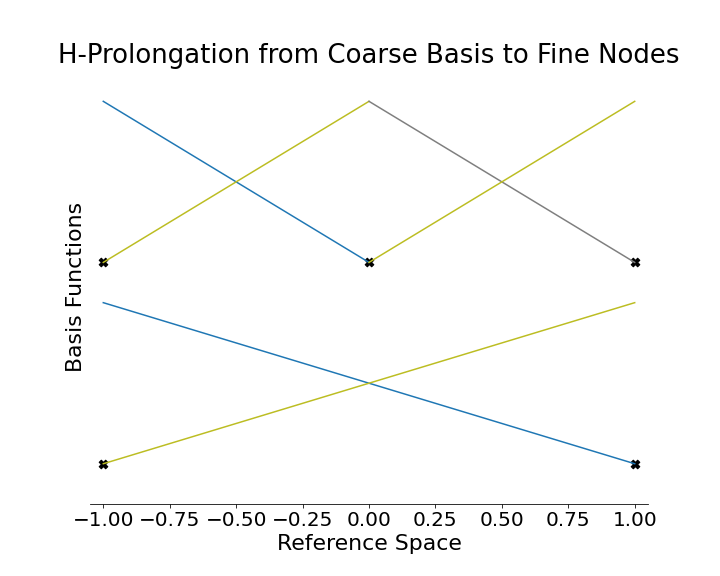
\includegraphics[width=0.48\textwidth]{../img/hProlongation}
  \caption{$H$-Prolongation from Coarse Basis to Fine Basis Points}
  \label{fig:h_prolongation}
\end{figure}

In Figure \ref{fig:h_prolongation}, we see an example of interpolation from a coarse grid basis to a fine grid macro-element basis.
The linear shape functions are evaluated at the nodes of the fine grid macro-element, which is a pair of linear sub-elements.
On the left linear sub-element, there are two basis functions which are zero over the domain of the right sub-element, and the reverse is also true.
The element level operator, ${\color{burgundy}\mathbf{A}}_e$, on the fine grid macro-element assembles the element level operator for each sub-element into the action of the PDE operator on the full macro-element.

With this macro-element structure, we can form the Fourier mode localization operator for the macro-element in the same fashion as the Fourier mode localization operator for high-order elements given in Equation \ref{eq:fouriermodelocalization1d}.
With macro-elements, there are $m p$ columns in the localization operator for a one dimensional scalar PDE on a macro-element with $m$ sub-elements instead of $p$ columns for a one dimensional scalar PDE on a single high order element.
\begin{equation}
\mathbf{Q} =
\begin{bmatrix}
    \mathbf{I}   \\
    \mathbf{e}_0 \\
\end{bmatrix} =
\begin{bmatrix}
    1      && 0      && \cdots && 0      \\
    0      && 1      && \cdots && 0      \\
    \vdots && \vdots && \vdots && \vdots \\
    0      && 0      && \cdots && 1      \\
    1      && 0      && \cdots && 0      \\
\end{bmatrix}
\end{equation}

Following the derivation from Section \ref{sec:lfahighorder}, we can derive the symbols of ${\color{burgundy}\mathbf{P}}_{\text{ctof}}$ and ${\color{burgundy}\mathbf{R}}_{\text{ftoc}}$.

\begin{definition}[Symbol of $H$-prolongation Operator]
The symbol of the $h$-prolongation operator is given by
\begin{equation}
\tilde{{\color{burgundy}\mathbf{P}}}_{\text{ctof}} \left( \boldsymbol{\theta} \right) = \mathbf{Q}_f^T \left( {\color{burgundy}\mathbf{P}}^e \odot \left[ e^{\imath \left( \mathbf{x}_{j, c} - \mathbf{x}_{i, f} \right) \cdot \mathbf{\theta} / \mathbf{h}} \right] \right) \mathbf{Q}_c
\end{equation}
where $i \in \left\lbrace 1, 2, \dots, n \left( m p + 1 \right)^d \right\rbrace$, $j \in \left\lbrace 1, 2, \dots, n \left( p + 1 \right)^d \right\rbrace$, $\mathbf{h}$ is the length of the macro-element, $d$ is the dimension of the finite element bases, $n$ is the number of components, and $m$ is the number of sub-elements in each fine grid macro-element.
The matrices $\mathbf{Q}_f$ and $\mathbf{Q}_c$ are the localization operators for the fine and coarse grid, respectively, and the macro-element $h$-prolongation operator is given by ${\color{burgundy}\mathbf{P}}^e = {\color{blue(ncs)}\mathbf{I}} {\color{applegreen}\mathbf{D}}_{\text{scale}} {\color{blue(ncs)}\mathbf{B}}_{\text{ctof}}$.
\label{def:h_prolongation_symbol}
\end{definition}

\begin{definition}[Symbol of $H$-restriction Operator]
The symbol of $h$-restriction operator is given by the expression
\begin{equation}
\tilde{{\color{burgundy}\mathbf{R}}}_{\text{ftoc}} \left( \boldsymbol{\theta} \right) = \mathbf{Q}_c^T \left( {\color{burgundy}\mathbf{R}}^e \odot \left[ e^{\imath \left( \mathbf{x}_{j, f} - \mathbf{x}_{i, c} \right) \cdot \boldsymbol{\theta} / \mathbf{h}} \right] \right) \mathbf{Q}_f
\end{equation}
where $i \in \left\lbrace 1, 2, \dots, n \left( p + 1 \right)^d \right\rbrace$, $j \in \left\lbrace 1, 2, \dots, n \left( m p + 1 \right)^d \right\rbrace$, $\mathbf{h}$ is the length of the macro-element, $d$ is the dimension of the finite element bases, $n$ is the number of components, and $m$ is the number of sub-elements in each fine grid macro-element.
The matrices $\mathbf{Q}_f$ and $\mathbf{Q}_c$ are the localization operators for the fine and coarse grid, respectively, and the macro-element $h$-restriction operator is given by ${\color{burgundy}\mathbf{R}}^e = {\color{burgundy}\mathbf{P}}^{e, T} = {\color{blue(ncs)}\mathbf{B}}_{\text{ctof}}^T {\color{applegreen}\mathbf{D}}_{\text{scale}} {\color{blue(ncs)}\mathbf{I}}$.
\label{def:h_restriction_symbol}
\end{definition}

\begin{figure}[!ht]
  \centering
  \subfloat[Spectrum of $H$-Multigrid for $p = 1$]{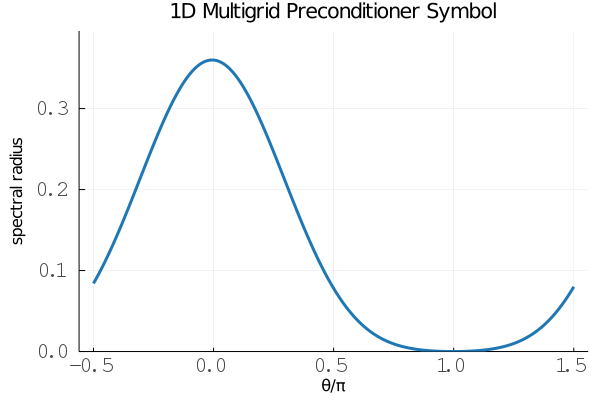
\includegraphics[width=0.48\textwidth]{../img/hmultigridSymbol1D}\label{fig:h_multigrid_spectrum_1d}}
  \hfill
  \subfloat[Spectrum of $H$-Multigrid for $p = 1$]{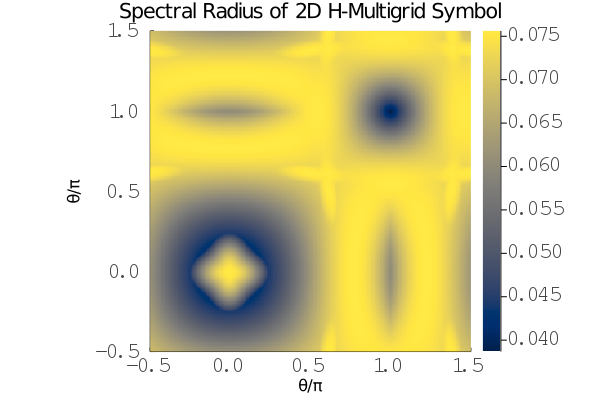
\includegraphics[width=0.48\textwidth]{../img/hmultigridSymbol2D}\label{fig:h_multigrid_spectrum_2d}}
  \caption{Spectrum of $H$-Multigrid Symbol for $p = 1$}
\end{figure}

In Figures \ref{fig:h_multigrid_spectrum_1d} and \ref{fig:h_multigrid_spectrum_2d}, we see the spectral radius of the symbol of $h$-multigrid for the scalar diffusion operator with third-order Chebyshev smoothing on a fine grid with a fourth-order $H^1$ Lagrange finite element basis and a coarse grid with a second-order $H^1$ Lagrange finite element basis on the Gauss-Lobatto points in one and two dimensions.
Various preconditioning techniques will reduce this spectral radius, with different effectiveness in different frequency ranges.
